\HydraSection[
  focus x=0.60,
  focus y=0.60,
  radius=0.13,
  zoom=2.05
]{The biological puzzle}

\HydraSubsection[
  A simple organism makes symmetry breaking directly visible.
]{Hydra as a model organism}

\begin{frame}{Hydra: simple body, continuous renewal}
  \HydraTextImage[5.60cm]{
    \HydraPoint
      {A small freshwater cnidarian}
      {A transparent, tube-shaped polyp attached to the substrate by a basal disc.}

    \HydraPoint
      {Simple oral--aboral anatomy}
      {A head with hypostome and tentacles, a body column, a budding zone and a foot.}

    \HydraPoint
      {Two epithelial layers}
      {Epidermis outside and gastrodermis inside, separated by mesoglea around one gastric cavity.}

    \HydraPoint
      {Continuous tissue renewal}
      {Stem cells divide in the body column while cells are displaced toward the head and foot.}

    \HydraPoint
      {Evolutionary significance}
      {An early-branching animal model for organizers, axial patterning and regeneration.}
  }{figures/hydra/hydra_staining.jpg}
  {Augustin R et al., Dev Biol. 2006; 296(1):62-70.}
\end{frame}

\begin{frame}{Hydra can rebuild a whole animal from very little}
  \HydraTextImage[5.60cm]{
    \HydraPoint
      {Head removal}
      {The remaining body column regenerates a new head at the wound.}

    \HydraPoint
      {Bisection}
      {The apical half rebuilds a foot; the basal half rebuilds a head --- producing two complete animals.}

    \HydraPoint
      {Small tissue fragment}
      {A fragment closes, rounds up, breaks symmetry and reconstructs an oral--aboral axis.}

    \HydraPoint[HydraCyan]
      {Dissociated cells}
      {Cells can be separated, reaggregated, sorted into layers and self-organized into new polyps.}

    \HydraPoint[HydraCyan]
      {The central puzzle}
      {Where does the new head form when the starting tissue is nearly symmetric?}
  }{figures/hydra/Hydra2.jpg}{Wittlieb J et al., Dev Biol. 2006; 296(1):62-70.}
\end{frame}

\begin{frame}{Regeneration unfolds through ordered stages}

  \begin{center}
    \begin{tikzpicture}
      \node[
        draw=HydraLine,
        rounded corners=4pt,
        inner sep=0.10cm
      ]{
        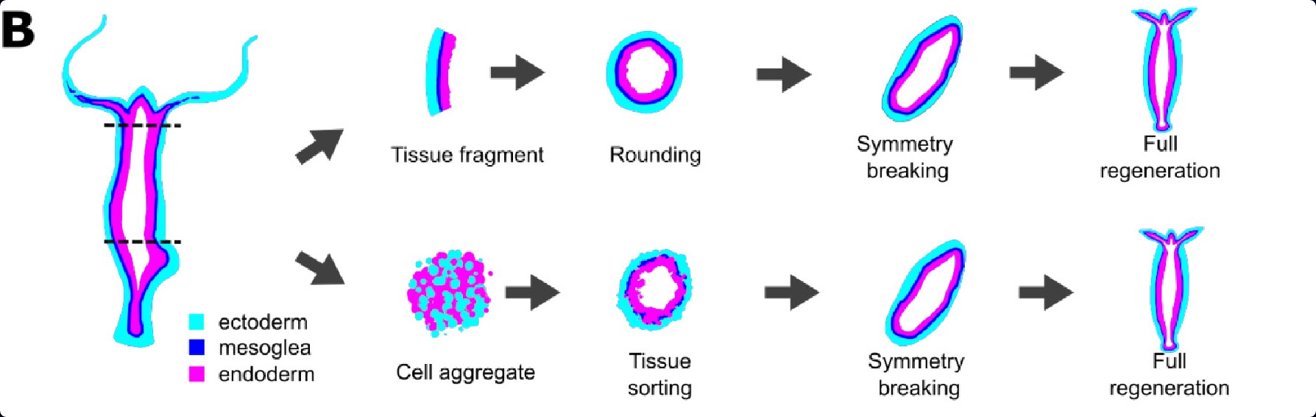
\includegraphics[
          width=0.94\textwidth,
          height=4.85cm,
          keepaspectratio
        ]{figures/hydra/hydra_regeneration_routes.png}
      };
    \end{tikzpicture}

    \vspace{0.04cm}

    {\color{HydraMuted}\fontsize{6}{7.2}\selectfont
      Wang, Bialas, Goel \& Collins,
      \textit{Integrative and Comparative Biology} 63 (2023), Fig.~1B.\par
    }
  \end{center}

  \vspace{0.12cm}

  \HydraTakeaway{
    Very different initial conditions pass through a similar spheroid stage
    before rebuilding a body axis
  }

\end{frame}


\begin{frame}{Symmetry breaks before a new head becomes visible}

  \begin{center}
    \begin{tikzpicture}
      \node[
        draw=HydraLine,
        rounded corners=4pt,
        inner sep=0.10cm
      ]{
        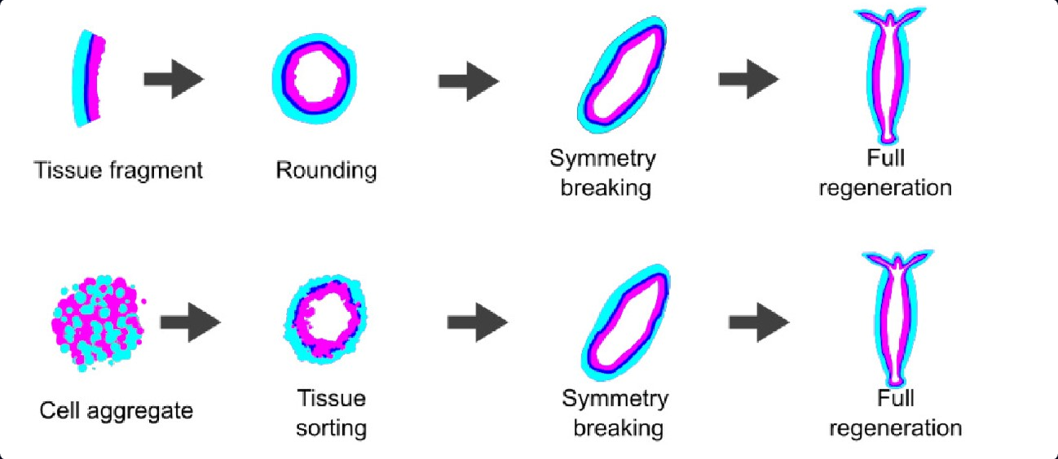
\includegraphics[
          width=0.80\textwidth,
          height=4.95cm,
          keepaspectratio
        ]{figures/hydra/hydra_symmetry_breaking_zoom.png}
      };
    \end{tikzpicture}

    \vspace{0.04cm}

    {\color{HydraMuted}\fontsize{6}{7.2}\selectfont
      Wang, Bialas, Goel \& Collins,
      \textit{Integrative and Comparative Biology} 63 (2023), Fig.~1B.\par
    }
  \end{center}

  \vspace{0.12cm}

  \HydraTakeaway{
    A local site acquires head-forming identity first; visible tentacles
    and the complete head--foot axis appear later
  }

\end{frame}

\HydraSubsection[
  Transplantation reveals that organizer activity depends on position and context.
]{Hydra grafting experiments}

\begin{frame}{A head graft can organize a second body axis}

  \begin{center}
    \begin{tikzpicture}
      \node[
        draw=HydraLine,
        rounded corners=4pt,
        inner sep=0.10cm
      ]{
        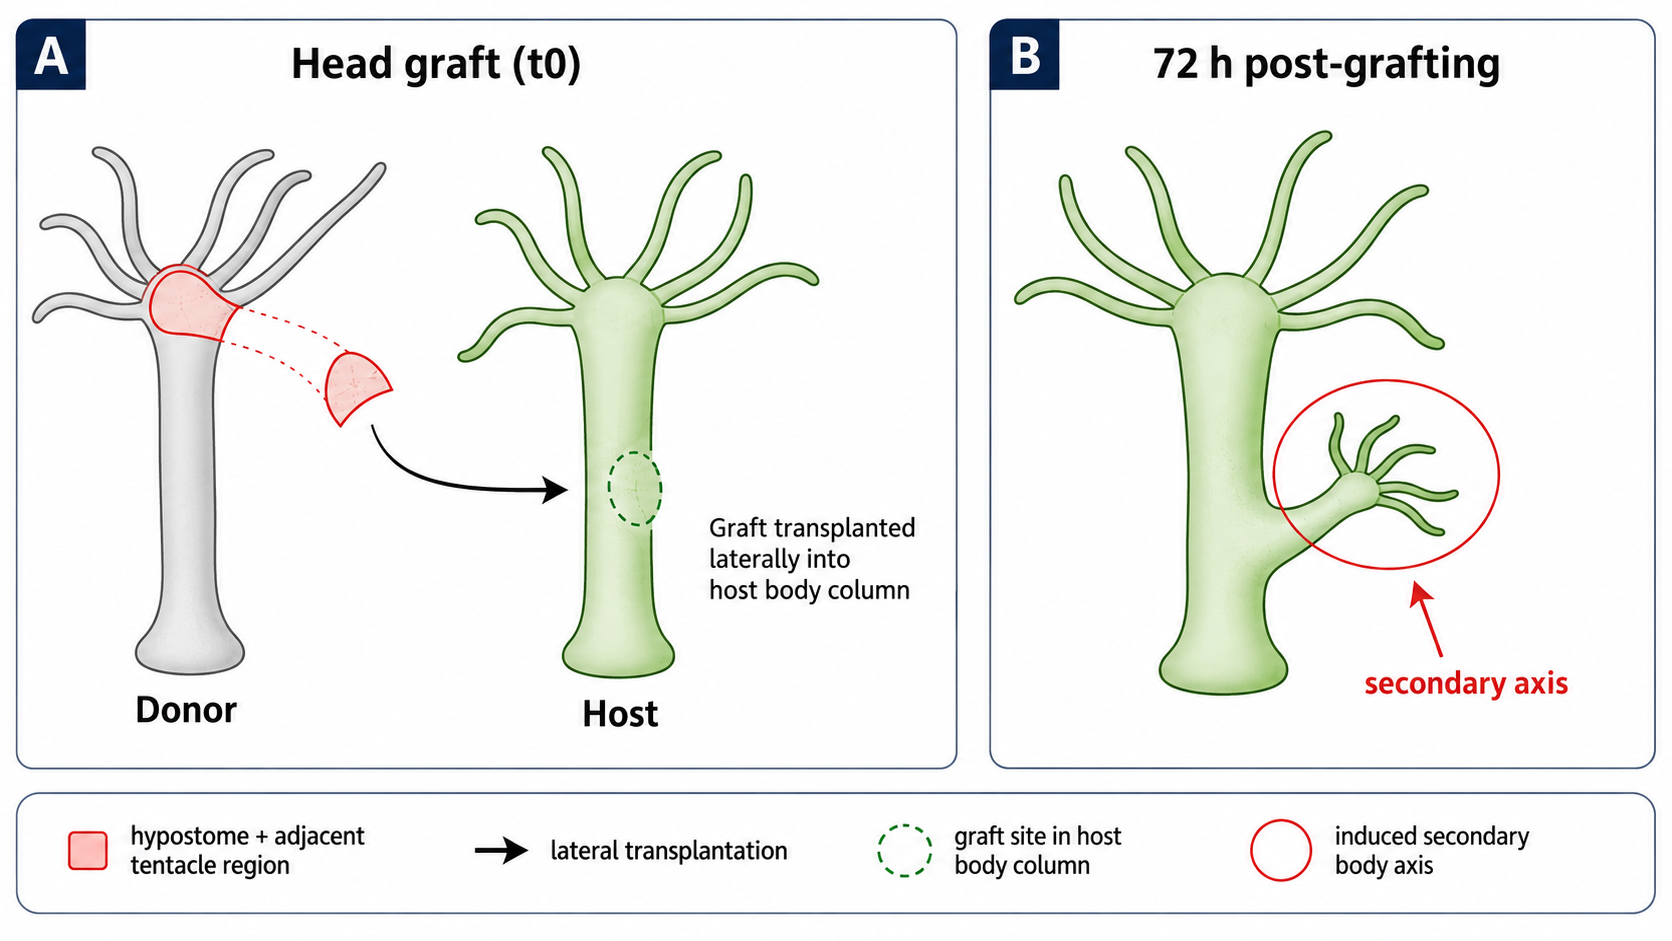
\includegraphics[
          width=0.92\textwidth,
          height=5.05cm,
          keepaspectratio
        ]{figures/hydra/a_clean_scientific_diagram_infographic_figure_wi_1.png}
      };
    \end{tikzpicture}

    \vspace{0.04cm}

    {\color{HydraMuted}\fontsize{6}{7.2}\selectfont
      Schematic based on the classic hypostome transplantation experiment
      of Browne (1909); see also Broun \& Bode (2002).\par
    }
  \end{center}

  \vspace{0.10cm}

  \HydraTakeaway{
    The graft does not simply grow into a second Hydra;
    it recruits a new body axis
  }

\end{frame}

\begin{frame}{Impact of the grafting position}

  \begin{center}
    \begin{tikzpicture}
      \node[
        draw=HydraLine,
        rounded corners=4pt,
        inner sep=0.10cm
      ]{
        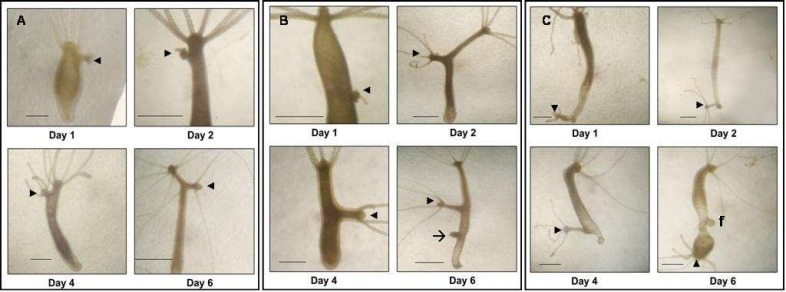
\includegraphics[
          width=0.92\textwidth,
          height=4.70cm,
          keepaspectratio
        ]{figures/hydra/grafting_timecourse.jpg}
      };
    \end{tikzpicture}

    \vspace{0.04cm}

    {\color{HydraMuted}\fontsize{6}{7.2}\selectfont
      Kadu, Ghaskadbi \& Ghaskadbi,
      \textit{Int. J. Mol. Cell. Med.}
      1 (2012).\par
    }
  \end{center}

  \vspace{0.10cm}

  \HydraTakeaway{
    The same graft can produce different outcomes depending on its position
  }

\end{frame}

\begin{frame}{Far from the host head: a complete second axis}

  \begin{columns}[T,onlytextwidth]

    \begin{column}{0.15\textwidth}
      \centering
      \begin{tikzpicture}[x=1cm,y=1cm]

        \draw[HydraCyan,line width=2pt] (0,0.35) -- (0,4.10);

        \fill[HydraGold] (0,4.10) circle[radius=0.09cm];
        \fill[HydraCyan] (0,0.35) circle[radius=0.09cm];

        \draw[HydraGold,line width=2pt]
          (-0.32,0.95) -- (0.32,0.95);

        \node[anchor=south,text=HydraGold,
          font=\bfseries\fontsize{5.8}{6.6}\selectfont]
          at (0,4.30) {HOST HEAD};

        \node[anchor=east,text=HydraGold,
          font=\bfseries\fontsize{5.8}{6.6}\selectfont]
          at (-0.38,0.95) {GRAFT};

        \node[anchor=north,text=HydraCyan,
          font=\bfseries\fontsize{5.8}{6.6}\selectfont]
          at (0,0.15) {HOST FOOT};

      \end{tikzpicture}

      \vspace{0.15cm}

      {\color{HydraMuted}\fontsize{6.2}{7.4}\selectfont
        lower host position\par}
    \end{column}

    \begin{column}{0.45\textwidth}
      \centering

      \begin{tikzpicture}
        \node[
          draw=HydraLine,
          rounded corners=4pt,
          inner sep=0.08cm
        ]{
          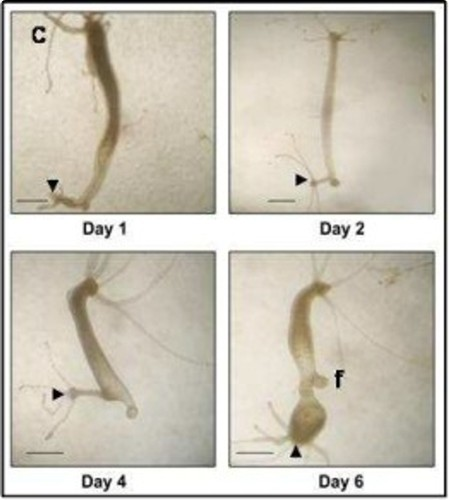
\includegraphics[
            width=\linewidth,
            height=4.65cm,
            keepaspectratio
          ]{figures/hydra/Bottom.jpg}
        };
      \end{tikzpicture}

      \vspace{0.04cm}

      {\color{HydraMuted}\fontsize{6}{7.2}\selectfont
        Kadu, Ghaskadbi \& Ghaskadbi,
        \textit{Int. J. Mol. Cell. Med.} 1 (2012), Fig.~2C.\par}
    \end{column}

    \begin{column}{0.34\textwidth}
      \vspace{0.5cm}
      \HydraPoint[HydraCyan]
        {A complete secondary axis}
        {The induced structure develops a foot, body column, hypostome and tentacles.}
      \vspace{0.7cm}
      \HydraPoint[HydraGold]
        {The strongest response}
        {Far from the host head, the same graft produces the longest and most complete secondary axis.}

    \end{column}

  \end{columns}

\end{frame}


\begin{frame}{Mid-body graft: an intermediate second axis}

  \begin{columns}[T,onlytextwidth]

    \begin{column}{0.15\textwidth}
      \centering
      \begin{tikzpicture}[x=1cm,y=1cm]

        \draw[HydraCyan,line width=2pt] (0,0.35) -- (0,4.10);

        \fill[HydraGold] (0,4.10) circle[radius=0.09cm];
        \fill[HydraCyan] (0,0.35) circle[radius=0.09cm];

        \draw[HydraGold,line width=2pt]
          (-0.32,2.25) -- (0.32,2.25);

        \node[anchor=south,text=HydraGold,
          font=\bfseries\fontsize{5.8}{6.6}\selectfont]
          at (0,4.30) {HOST HEAD};

        \node[anchor=east,text=HydraGold,
          font=\bfseries\fontsize{5.8}{6.6}\selectfont]
          at (-0.38,2.25) {GRAFT};

        \node[anchor=north,text=HydraCyan,
          font=\bfseries\fontsize{5.8}{6.6}\selectfont]
          at (0,0.15) {HOST FOOT};

      \end{tikzpicture}

      \vspace{0.15cm}

      {\color{HydraMuted}\fontsize{6.2}{7.4}\selectfont
        middle host position\par}
    \end{column}

    \begin{column}{0.45\textwidth}
      \centering

      \begin{tikzpicture}
        \node[
          draw=HydraLine,
          rounded corners=4pt,
          inner sep=0.08cm
        ]{
          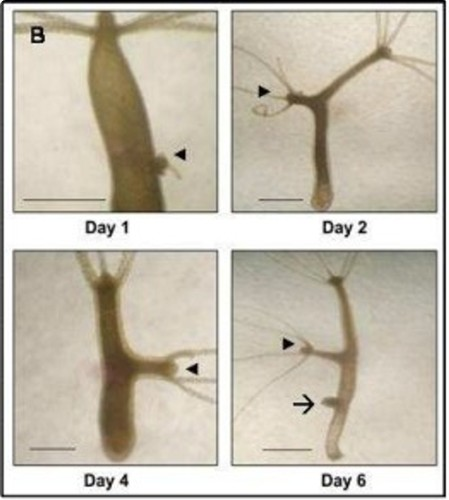
\includegraphics[
            width=\linewidth,
            height=4.65cm,
            keepaspectratio
          ]{figures/hydra/Middle.jpg}
        };
      \end{tikzpicture}

      \vspace{0.04cm}

      {\color{HydraMuted}\fontsize{6}{7.2}\selectfont
        Kadu, Ghaskadbi \& Ghaskadbi,
        \textit{Int. J. Mol. Cell. Med.} 1 (2012), Fig.~2B.\par}
    \end{column}

    \begin{column}{0.34\textwidth}
      \vspace{0.5cm}
      \HydraPoint[HydraCyan]
        {An intermediate secondary axis}
        {The induced axis grows substantially longer than after an upper-body graft.}
      \vspace{0.7cm}
      \HydraPoint[HydraGold]
        {Only position has changed}
        {The donor tissue is the same; moving the graft along the host axis changes the resulting morphology.}

    \end{column}

  \end{columns}

\end{frame}


\begin{frame}{Near the host head: only a short second axis}

  \begin{columns}[T,onlytextwidth]

    \begin{column}{0.15\textwidth}
      \centering
      \begin{tikzpicture}[x=1cm,y=1cm]

        \draw[HydraCyan,line width=2pt] (0,0.35) -- (0,4.10);

        \fill[HydraGold] (0,4.10) circle[radius=0.09cm];
        \fill[HydraCyan] (0,0.35) circle[radius=0.09cm];

        \draw[HydraGold,line width=2pt]
          (-0.32,3.35) -- (0.32,3.35);

        \node[anchor=south,text=HydraGold,
          font=\bfseries\fontsize{5.8}{6.6}\selectfont]
          at (0,4.30) {HOST HEAD};

        \node[anchor=east,text=HydraGold,
          font=\bfseries\fontsize{5.8}{6.6}\selectfont]
          at (-0.38,3.35) {GRAFT};

        \node[anchor=north,text=HydraCyan,
          font=\bfseries\fontsize{5.8}{6.6}\selectfont]
          at (0,0.15) {HOST FOOT};

      \end{tikzpicture}

      \vspace{0.15cm}

      {\color{HydraMuted}\fontsize{6.2}{7.4}\selectfont
        upper host position\par}
    \end{column}

    \begin{column}{0.45\textwidth}
      \centering

      \begin{tikzpicture}
        \node[
          draw=HydraLine,
          rounded corners=4pt,
          inner sep=0.08cm
        ]{
          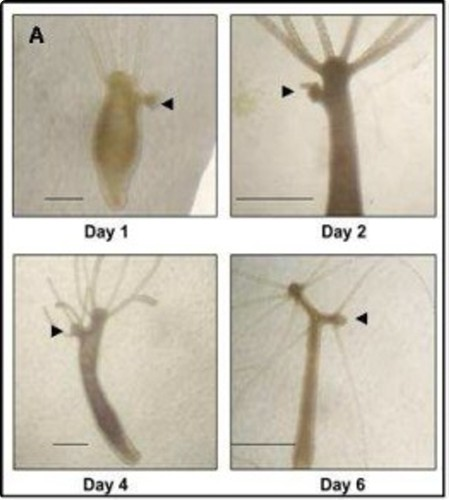
\includegraphics[
            width=\linewidth,
            height=4.65cm,
            keepaspectratio
          ]{figures/hydra/Top.jpg}
        };
      \end{tikzpicture}

      \vspace{0.04cm}

      {\color{HydraMuted}\fontsize{6}{7.2}\selectfont
        Kadu, Ghaskadbi \& Ghaskadbi,
        \textit{Int. J. Mol. Cell. Med.} 1 (2012), Fig.~2A.\par}
    \end{column}

    \begin{column}{0.34\textwidth}
      \vspace{0.5cm}
      \HydraPoint[HydraCyan]
        {A very short secondary axis}
        {The hypostome graft still induces a new head, but only a short body column develops.}
      \vspace{0.7cm}
      \HydraPoint[HydraGold]
        {Growth is strongly constrained}
        {Close to the host head, the induced axis remains small despite using the same organizer tissue.}

    \end{column}

  \end{columns}

\end{frame}


\begin{frame}{Multiple grafts can impose multiple axes}

  \begin{columns}[T,onlytextwidth]

    \begin{column}{0.47\textwidth}

      \vspace{0.9cm}

      \HydraPoint
        {Three grafts on one host}
          {A complete foot was grafted in the upper region, hypostome pieces were grafted in the middle and lower regions.}


      \vspace{0.3cm}

      \HydraPoint[HydraCyan]
        {Three secondary axes}
        {All three grafted regions produced an induction simultaneously.}

      \vspace{0.3cm}

      \HydraPoint
        {Organizer identity matters}
        {The axes induced by hypostome tissue were substantially longer than the axis induced by the foot graft.}


    \end{column}

    \begin{column}{0.49\textwidth}

      \centering

      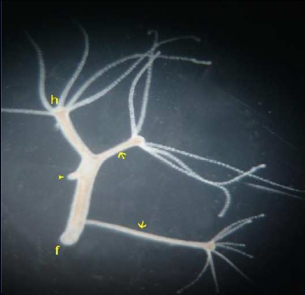
\includegraphics[
        width=\linewidth,
        height=5.55cm,
        keepaspectratio
      ]{figures/hydra/Multiple.png}

      \vspace{0.05cm}

      {\color{HydraMuted}\fontsize{6}{7.2}\selectfont
        Kadu, Ghaskadbi \& Ghaskadbi,
        \textit{Int. J. Mol. Cell. Med.} 1 (2012), Fig.~6.\par}

    \end{column}

  \end{columns}

  \vspace{0.20cm}

  \begin{center}
    \begin{minipage}{0.78\textwidth}
      \centering
      {\color{HydraGold}\bfseries\fontsize{9.0}{11.2}\selectfont
        Multiple local organizers can coexist and impose
        several body axes on the same tissue.\par}
    \end{minipage}
  \end{center}

\end{frame}





\begin{frame}{From experiments to a mathematical model}

  \vspace{0.20cm}
  \HydraProcess
    {regenerating tissue}
    {organizer selection}
    {one body axis}

  \vspace{0.40cm}

  \HydraProcess
    {ectopic organizer}
    {interaction with host}
    {secondary axis}

  \vspace{0.95cm}

  % ------------------------------------------------------------
  % Row 1
  % ------------------------------------------------------------
  \begin{columns}[T,onlytextwidth]

    \begin{column}{0.47\textwidth}
      \begin{minipage}[t][1.55cm][t]{\linewidth}
        \vspace{0pt}
        \HydraPoint[HydraGold]
          {Spontaneous pattern formation}
          {How can a localized organizer emerge from weakly patterned or nearly symmetric tissue?}
      \end{minipage}
    \end{column}

    \begin{column}{0.47\textwidth}
      \begin{minipage}[t][1.55cm][t]{\linewidth}
        \vspace{0pt}
        \HydraPoint[HydraGold]
          {Organizer induction}
          {Why can a transplanted organizer recruit host tissue and initiate a new axis?}
      \end{minipage}
    \end{column}

  \end{columns}

  \vspace{0.38cm}

  % ------------------------------------------------------------
  % Row 2
  % ------------------------------------------------------------
  \begin{columns}[T,onlytextwidth]

    \begin{column}{0.47\textwidth}
      \begin{minipage}[t][1.55cm][t]{\linewidth}
        \vspace{0pt}
        \HydraPoint[HydraGold]
          {Competition and uniqueness}
          {Why does normal regeneration usually select one head, while several grafts can sustain several axes?}
      \end{minipage}
    \end{column}

    \begin{column}{0.47\textwidth}
      \begin{minipage}[t][1.55cm][t]{\linewidth}
        \vspace{0pt}
        \HydraPoint[HydraGold]
      {Context dependence}
      {Why does the same hypostome graft produce different secondary axes at different positions in the host?}
      \end{minipage}
    \end{column}

  \end{columns}

  \vfill

  % \HydraTakeaway{
  %   A mathematical model should capture both self-organization
  %   and the response to an imposed organizer.
  % }

\end{frame}